\section{Résumé d'activité des semaines 38-39}

Durant ces deux semaines, nous avons entamé le développement des différents acteurs de notre projet Tower Defense. Nous avons profité de cette période pour approfondir nos connaissances en C++, notamment sur des notions essentielles telles que les pointeurs, les classes et l’héritage, les structures, les tableaux statiques et dynamiques, ainsi que la syntaxe générale. Nous nous sommes également intéressés à la manière de faire interagir nos différents acteurs (par exemple, les ennemis et les tourelles affichés dans une fenêtre SFML, ainsi que leurs comportements respectifs).

Afin de progresser efficacement, nous avons choisi de travailler chacun sur un programme distinct. Ce choix nous a semblé pertinent, car il permettait à chacun d’apprendre de manière autonome les bases indispensables au projet. Toutefois, cette répartition n’a pas empêché une réelle coopération : nous avons régulièrement partagé nos découvertes et nous nous sommes mutuellement aidés lorsque l’un d’entre nous rencontrait des difficultés.

Ce rapport propose un résumé de nos activités durant cette période. La première partie est consacrée aux travaux réalisés par Alexandre TECHER, tandis que la seconde présente ceux d’Enzo CHADEVILLE. Enfin, nous terminerons par une conclusion mettant en perspective ces deux semaines de travail et notre vision pour la suite du projet.

\section{Alexandre TECHER}
%

\subsection{Classes}

\subsubsection{Classe Enemy}
\paragraph{}
La classe Enemy représente les ennemis dans le jeu. Elle gère les attributs tels que la santé, la vitesse, et la position. Elle inclut également des méthodes pour déplacer les ennemis le long du chemin défini par l'algorithme de "chemin le plus court".

Elle contient une structure "enemy" qui regroupes les informations décrivant un ennemi (nom, forme (shape), position, vie, vitesse, carapace, attaque, vitesse d'attaque, portée, pathPoints, currentPathIndex, nombre d'ennemis).


"pathPoints" est un vecteur de sf::Vector2f qui contient les points du chemin que l'ennemi doit suivre. "currentPathIndex" est un entier qui indique l'index actuel dans le vecteur pathPoints.


Spawn Position() : Cette méthode initialise la position de l'ennemi sur la carte de manière aléatoire.

Move() : Cette méthode déplace l'ennemi le long du chemin défini par les points dans pathPoints. Elle utilise la vitesse de l'ennemi pour déterminer la distance à parcourir à chaque mise à jour.
Grâce à la boucle "while", la fonction move() est exécutée en continue. Ainsi SolveAStar() est appelé régulièrement pour recalculer le chemin de l'ennemi en fonction de sa position actuelle.


Draw() : Cette méthode dessine l'ennemi à sa position actuelle sur la fenêtre de jeu.


Pour contenir les caractéristiques et le chemin de chaque ennemi, un vecteur "groupe\_enemies" est utilisé. Chaque élément du vecteur est une instance de la structure "enemy".


\subsection{Classe Tower}
\paragraph{}

La classe Tower représente les tours que le joueur peut placer sur la carte. Elle gère les attributs tels que le type de tour, les dégâts, la portée, et le coût. Elle inclut des méthodes pour attaquer les ennemis lorsqu'ils entrent dans sa portée.


\subsection{Classe Pathfinding AStar}
\paragraph{}

Afin de permettre aux ennemis de se déplacer de manière intelligente sur la carte, un algorithme de pathfinding est nécessaire.
Dans un premier temps, une lecture de la description de la librairie boost_graph a permis de cerner les algorithmes de pathfinding disponibles.

lien de descriptionn: \url{https://www.boost.org/doc/libs/latest/libs/graph/doc/index.html}

L'algoritme Dijkstra's Shortest Paths a été envisagé. Mais après réflexion et comparaison sur wikipédia, l'algorithme A* (A-star) a été préféré car il est généralement plus efficace pour les jeux vidéo et les applications en temps réel.


La classe Pathfinding AStar implémente l'algorithme A* pour trouver le chemin le plus court entre deux points sur la carte.
Elle est utilisée par la classe Enemy pour déterminer le chemin à suivre.


Tout d'abord, le programme de A* est inspiré du github suivant : 


\url{https://github.com/OneLoneCoder/Javidx9/blob/master/ConsoleGameEngine/SmallerProjects/OneLoneCoder_PathFinding_AStar.cpp}


La vidéo suivante explique le fonctionnement de l'algorithme A* : 


\url{https://www.youtube.com/watch?v=icZj67PTFhc} 


Après modification du code source pour une utilisation avec SFML, l'algorithme A* fonctionne de la manière suivante :
\begin{itemize}


    \item La carte est représentée comme une grille de nœuds, où chaque nœud correspond à une cellule de la carte. 
    Chaque nœud a des attributs tels que son état (libre ou occupé), ses coordonnées, 
    le coût pour atteindre ce nœud depuis le nœud de départ, le coût estimé pour atteindre le nœud d'arrivée depuis ce nœud, 
    un vecteur contenant ses voisins, et un pointeur qui sera dirigé vers son noeud parent.


    \item CreateNodes() : Cette méthode initialise la grille de nœuds en fonction de la carte du jeu. 
    Elle créé des nœuds pour chaque cellule de la carte et définit leurs attributs initiaux.
    

    \item EnemyNode() : Cette méthode traduit la position actuelle de l'ennemi en coordonnées de nœud dans la grille.
    Elle n'est pas forcément située au centre d'un nœud.


    \item SolveAStar() : C'est la méthode principale qui implémente l'algorithme A*. Elle prend en entrée les coordonnées de l'ennemi,
    et retourne un vecteur de nœuds représentant le chemin le plus court trouvé.
    

    \item Draw() : Cette méthode est utilisée pour visualiser la grille de nœuds et le chemin trouvé.
    Elle dessine chaque nœud avec une couleur différente en fonction de son état, et trace le chemin en reliant les nœuds du chemin trouvé.


\end{itemize}

Le résultat obtenu après l'exécution de l'algorithme A* est figuré ci-dessous :

\begin{figure}[h]
\centering
    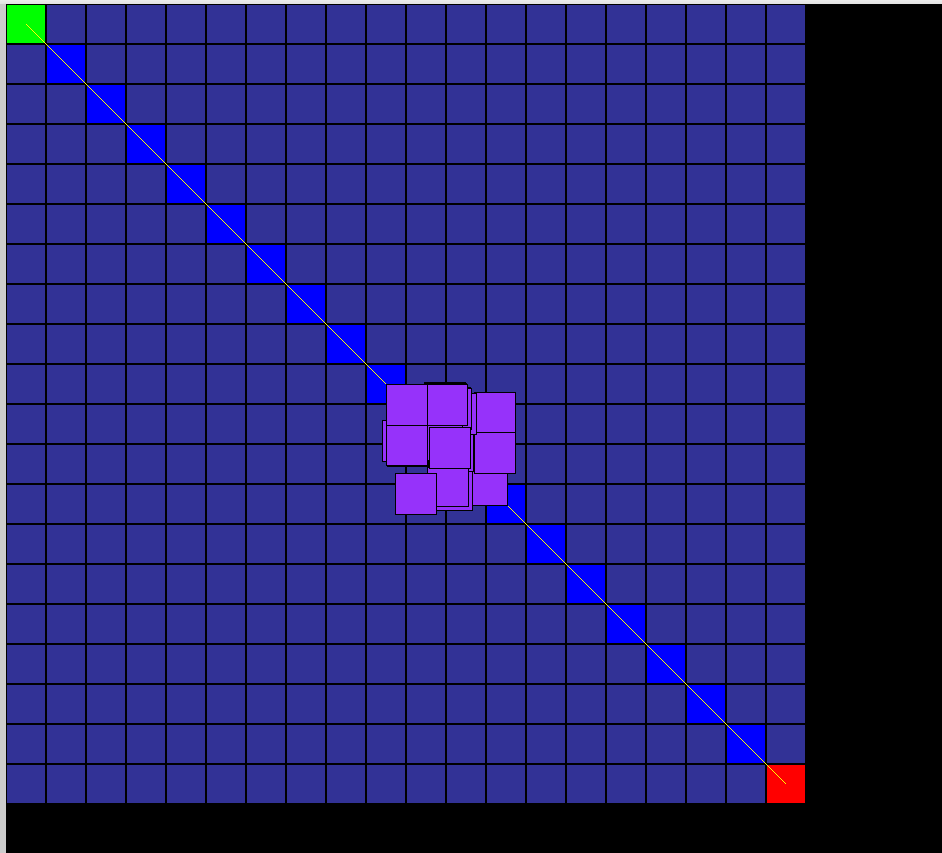
\includegraphics[width=0.7\textwidth]{figs/ASTAR.png}
    \caption{Déplacement des ennemis avec l'algorithme A*}
\end{figure}

\newpage

\paragraph{}

Le chemin le plus court est représenté par une ligne jaune reliant les nœuds verts (noeud de départ) et rouge (nœud d'arrivée).
Les nœuds bleus claires représentent les nœuds libres visités par l'algorithme, tandis que les nœuds bleus foncés représentent les nœuds libres non visités.


Ici, seulement un noeud est vert, car on affiche le noeud de départ du premier ennemi apparu.


\subsection{Difficulés rencontrées}
\paragraph{}
Les principales difficultés rencontrées à ce stadde du projet ont été les suivantes :


\item La mise en place de l'algorithme A* pour le pathfinding des ennemis. Cela a nécessité une compréhension approfondie de l'algorithme et son adaptation à la librairie SFML.
\item l'échange de données entre les différentes classes, notamment entre la classe Enemy et la classe Pathfinding AStar.
\item la définition et la gestion du movement fluide des ennemis le long du chemin calculé par l'algorithme A*.

Important : Après plusieurs tentatives de résolution, ChatGPT a été utilisé pour résoudre certaines erreurs de compilation mais aussi pour surmonter les difficultés lors de la création de A* et du mouvement des ennemis.

\subsection{Pistes d'amélioration}
\paragraph{}

La structure des ennemis peut être remplacée par des classes dérivées pour chaque type d'ennemi. Cela permettrait une meilleure organisation du code et une plus grande flexibilité pour ajouter de nouveaux types d'ennemis avec des comportements spécifiques.


La création de tours devra être implémentée, avec des classes dérivées pour chaque type de tour. Chaque classe de tour pourrait avoir des attributs et des méthodes spécifiques, comme le type de dégâts infligés, la portée, et la vitesse d'attaque.


A* devra prendre en compte les tours placées par le joueur pour recalculer le chemin des ennemis en temps réel. Cela ajouterait une dimension stratégique au jeu, car les joueurs pourraient influencer le chemin des ennemis en plaçant des tours de manière stratégique.

De plus, au lieu de prendre en compte qu'un seul noeud de fin, A* pourrait être modifié pour prendre en compte plusieurs noeuds de fin, représentant plusieurs points d'arrivée possibles pour les ennemis.

Cela permettrait aux ennemis de choisir le chemin le plus court vers n'importe quel point d'arrivée.

\newpage

%%%%%%%%%%%%%%%%%%%%%%%%%%%%%%%%%%%%%%%%%%%%%%%%%%%%%%%%%%%%%%%%%%%%%%%%%%%%%%%%%%%%%%%%%%%%%%%%%%%%%%%%%%%%%%%%%%%%%%%%%%%%%%%%%%%%%%%%%%%%%%%%%%%%%%%%%%%%%%%%%%%%%%%%%%%%%%%%%%%%%%%%%%%%Ù

\newpage

\section{Enzo CHADEVILLE}
\subsection{Les classes}

Durant ces deux semaines, j’ai majoritairement travaillé sur l’apprentissage des classes et des classes héritières. La quasi-totalité de la semaine 38 a été utilisée pour comprendre concrètement comment ces classes peuvent communiquer. J’ai d’abord cherché à établir plusieurs types d’ennemis, définir arbitrairement leurs statistiques, réfléchir aux variables qui nous seraient utiles pour le jeu, déterminer ce que je devais mettre dans le constructeur, comment stocker mes ennemis, etc.

\begin{figure}[h]
    \centering
    \makebox[\textwidth]{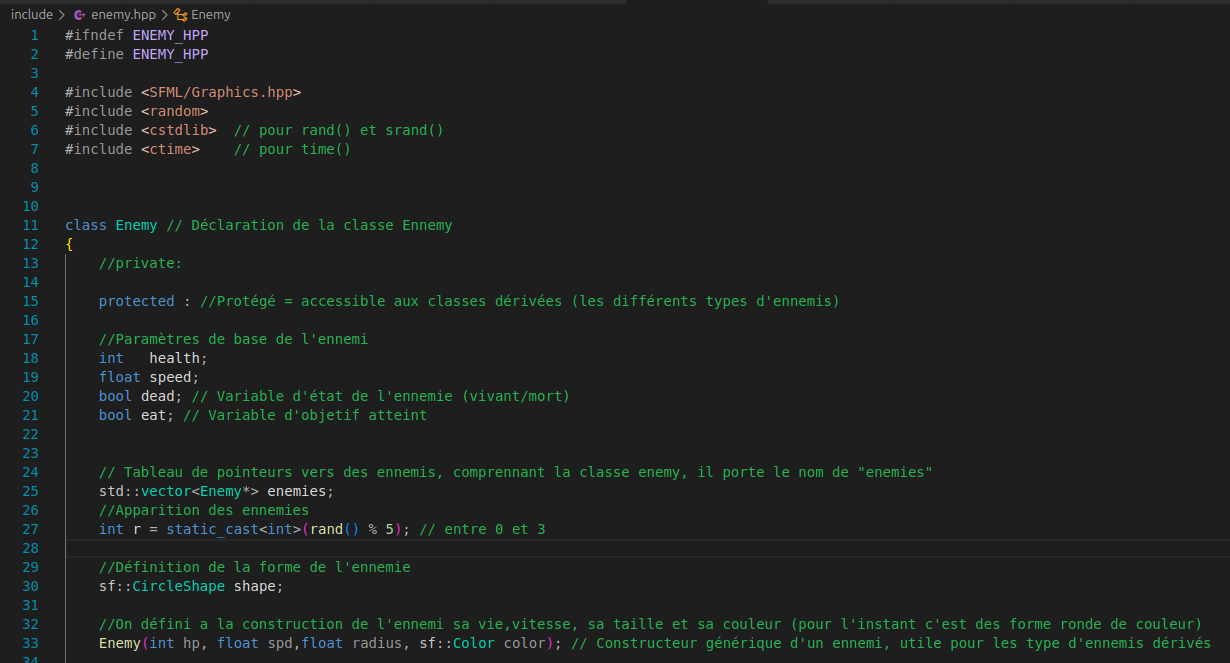
\includegraphics[width=1\textwidth]{figs/CLASSEE1.png}}
    \caption{"enemy.hpp" – Classe Enemy, déclaration et partie \texttt{protected}}
    \label{fig:exemple}
\end{figure}

Sur l’ensemble de mes programmes, j’ai cherché à commenter la fonction de chaque ligne. Prendre rapidement cette habitude m’a permis de mieux me repérer dans mes fonctions, et de mieux comprendre le fonctionnement de certaines méthodes incluses dans les librairies SFML ou encore les constructeurs. J’ai également « archivé » des parties de programme qui ne fonctionnaient pas ou qui ne me servaient plus.  
Sur la figure 1 se trouve la déclaration et le début de la classe « maîtresse ». Cette classe Enemy constituera la base de nos ennemis. On donne donc au constructeur certaines informations récurrentes nécessaires à tous les ennemis, à savoir leur vie, leur vitesse, leur taille et leur couleur pour l’affichage dans SFML. Nous pourrons implémenter au besoin plusieurs fonctions supplémentaires assez facilement.

\begin{figure}[h]
    \centering
    \makebox[\textwidth]{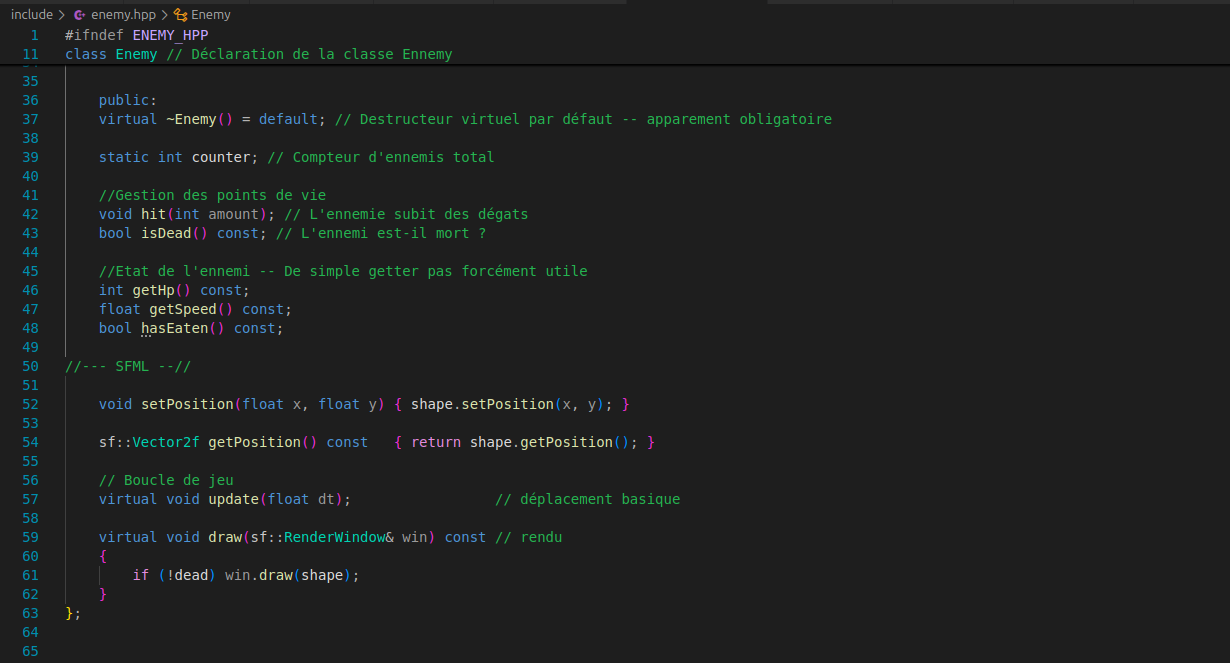
\includegraphics[width=1\textwidth]{figs/CLASSEE2.png}}
    \caption{"enemy.hpp" – Classe Enemy, partie \texttt{public}, fonctions généralisées}
    \label{fig:exemple}
\end{figure}

\newpage

Dans la partie publique de la classe Enemy, je déclare les fonctions qui permettront de gérer les ennemis. J’ai également implémenté la fonction de compteur que nous avons vue en cours pour calculer le nombre d’ennemis. Pour l’instant, elle ne nous sert pas à grand-chose, puisque Alexandre et moi ne nous basons pas sur cette variable pour suivre nos ennemis. Ne m’étant pas encore occupé de la partie pathfinding, les ennemis n’ont pas de comportement complexe : seule leur forme et leur apparition sur une carte sont gérées.

Voici un exemple de quelques classes héritières de Enemy. Pour l’instant, je n’ai pas implémenté de fonctions propres à ces classes, mais on constate que, grâce à leur constructeur, je peux modifier manuellement les paramètres de la classe héritière. Ce système est vraiment intéressant, car il permet de créer différents types d’ennemis avec de simples variations de statistiques. Lorsque nous aurons suffisamment avancé, nous ajouterons des fonctions internes. Pour le moment, le fait de les différencier uniquement par leurs statistiques nous montre déjà que, grâce à une classe de base, nous pouvons générer une grande variété de déclinaisons.

J’ai pris la décision de déclarer les statistiques des ennemis directement dans le constructeur plutôt qu’au moment de leur génération. L’avantage est que la déclaration est centralisée dans un seul endroit et rend explicite le fait que les ennemis d’une classe donnée, comme FastEnemy, sont tous identiques.

\newpage

\begin{lstlisting}
//----------------------------------------------------------
// Ennemi tank (comportement identique aux ennemis de base,
// hp et vitesse changent)

class TankEnemy : public Enemy
{
public:
    static int counter; // Compteur d'ennemis de type TankEnemy
    TankEnemy() : Enemy(300, 1, 10.f, sf::Color(0,0,255)) { ++counter; }
    ~TankEnemy() { --TankEnemy::counter; } 
};

//----------------------------------------------------------
// Ennemi target (objectif : détruire les tourelles sur leur passage
// chemin le plus court en ignorant les tourelles, hp et vitesse changent)

class TargetEnemy : public Enemy
{
public:
    static int counter; // Compteur d'ennemis de type TargetEnemy
    TargetEnemy() : Enemy(150, 3, 4.f, sf::Color(100,100,100)) { ++counter; }
    ~TargetEnemy() { --TargetEnemy::counter; }
};
\end{lstlisting}

J’ai pu réutiliser ce squelette pour mes tours en changeant simplement les noms, il n’y a pas eu de difficulté notable sur la création des tours.

\newpage

\subsection{L’affichage}

Pour l’instant l’affichage en SFML se fait sur deux fichiers, le \texttt{main.cpp} et le \texttt{render.cpp}. L’idée à terme est que toute la gestion du SFML soit gérée dans le fichier \texttt{render.cpp} afin de rendre le code plus propre, mais aussi de « nettoyer » le main pour n’y importer que les fonctions essentielles du genre \texttt{Game start}.  

Ici le main gère l’initialisation du programme, c’est-à-dire la création de la fenêtre, l’initialisation des tableaux de pointeurs de type classe importante. On remarque le tableau de pointeurs de la classe Enemy : concrètement cette fonction permet de faire un tableau avec l’intégralité de nos ennemis, même si ce sont des classes héritières. Cela fonctionne parce qu’elles découlent toutes de la classe Enemy, ce qui est super pratique. Je pense qu’à terme nous fonctionnerons comme ça pour stocker nos ennemis, car il nous suffira de récupérer un identifiant de l’ennemi pour savoir à quelle espèce il appartient.  
On pourrait également faire plusieurs tableaux par espèce d’ennemis, mais si je dois me projeter je pense qu’en créer un par ennemi nous poserait des difficultés dans le cas où nous aurions besoin de faire une tourelle à AOE. En plus de cela, cela obligerait à effectuer toutes les actions de rendu et de traitement des ennemis globaux en N* par type d’ennemi, ce qui n’est selon moi pas très pratique.  

On fait également la même chose pour les tourelles puisque nous allons nous en servir de la même façon que pour les ennemis.

\begin{lstlisting}
int main() {

//------------- INITIALISATION ---------------//

    // Initialisation de la fenêtre SFML
    sf::RenderWindow game_window(sf::VideoMode(800, 600), "Enemies + SFML");
    game_window.setFramerateLimit(60);

    // Initialisation des acteurs
    std::vector<Enemy*> enemies;      // PAS de new ici, pas besoin grâce à l’instance de Game
    std::vector<Tourelle*> tourelles; // PAS de new ici, pas besoin grâce à l’instance de Game
    std::vector<Render::Cell> cells;  // Tableau de cellules pour la grille
    cells = Render::buildCells(game_window); // On construit les cellules une fois pour toutes au début
    Game game;                       

    // Initialisation des aléatoires
    std::srand(static_cast<unsigned>(std::time(nullptr))); // seed une fois

    // Initialisation d’une clock
    sf::Clock clock;
    const float spawnoffset = 0.5f; // spawn toutes les 0.5s
\end{lstlisting}

\newpage

Pour pouvoir gérer le jeu efficacement, j’ai pris la décision de faire dessiner une grille sur la fenêtre. Je vais me servir de cette grille pour faire apparaître des ennemis et des tourelles sur certaines cases.  
L’avantage de ça, c’est que ça rend selon moi plus pratique la pose de tourelle : plutôt que de dire « Je pose une tourelle au pixel (x,y) » et risquer de pouvoir poser une tourelle juste à côté au pixel voisin, ici on définit directement la taille d’une case.  
Pour faire une analogie, ce serait comme lorsque l’on place une structure dans *Clash of Clans* (ou n’importe quel jeu de gestion à grille comme *Age of Empires*), ou même *Minecraft* pour les jeux de survie.  

\begin{figure}[h]
    \centering
    \makebox[\textwidth]{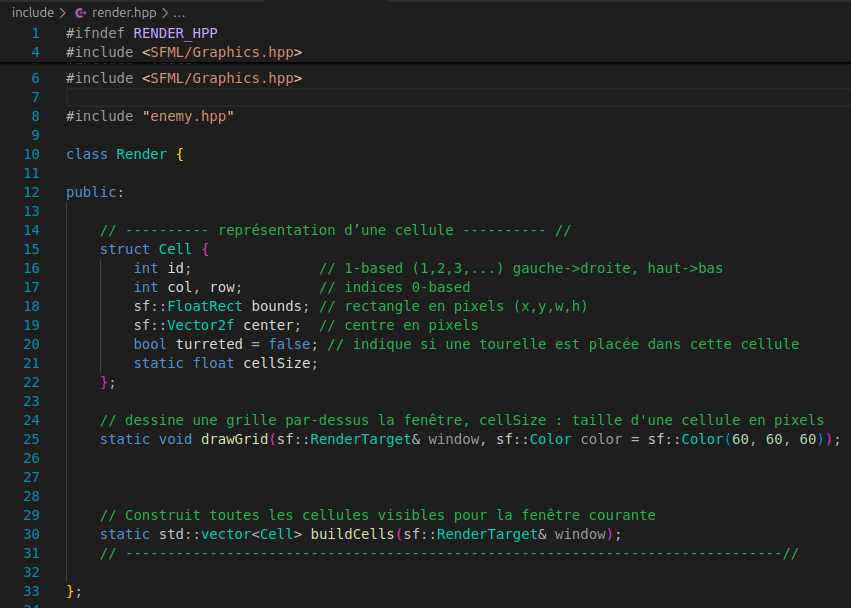
\includegraphics[width=1\textwidth]{figs/CELLS1.png}}
    \caption{"render.hpp" – Classe Render, partie \texttt{public}, fonctions de la grille}
    \label{fig:exemple}
\end{figure}

\newpage

Cependant, je ne pouvais pas (par souci de structure du programme) faire à la fois la fonction de dessin et la génération de mon tableau de cellules (j’appelle cellule une case dans la grille). J’ai donc dû les séparer.  

La fonction « buildCells » est donc la fonction « pratique », c’est elle qui possède toutes les caractéristiques de ma cellule.  
Ma cellule comporte les caractéristiques suivantes :


\begin{figure}[h]
    \centering
    \makebox[\textwidth]{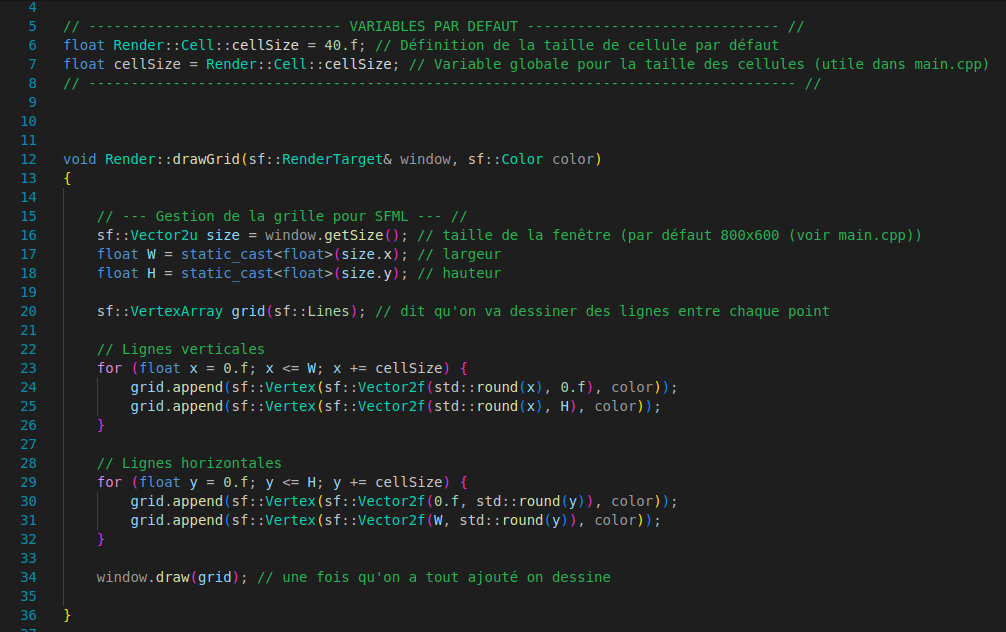
\includegraphics[width=0.8\textwidth]{figs/drawgrid.png}}
    \caption{"render.hpp" – Classe Render, fonctions, drawGrid}
    \label{fig:exemple}
\end{figure}

\begin{figure}[h]
    \centering
    \makebox[\textwidth]{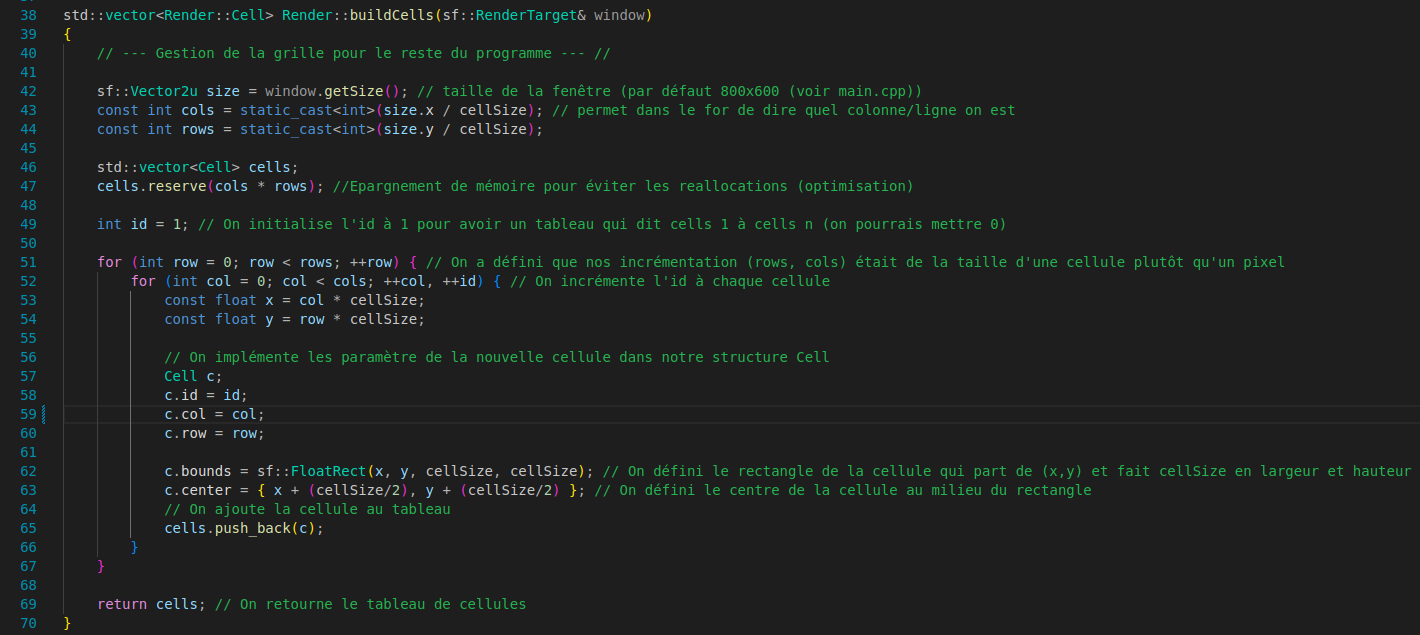
\includegraphics[width=0.8\textwidth]{figs/buildcells.png}}
    \caption{"render.cpp" – Classe Render, fonctions, buildCells}
    \label{fig:exemple}
\end{figure}


On a donc l’id qui permet d’identifier chaque cellule, row et col qui servent au calcul de leurs coordonnées, center qui permet d’indiquer les coordonnées x,y du centre de celle-ci, un booléen turreted qui permet de voir si une cellule a déjà une tourelle installée dessus (avantage : évite les empilements sur une seule cellule et rend l’affichage plus propre). Enfin, une variable « static » cellSize indique que chaque instance de cette structure possède la même taille, ce qui est pratique pour standardiser un processus.  
Enfin, les deux fonctions : « drawGrid », qui s’occupe du visuel, et « buildCells » pour le côté pratique.  

Les deux fonctions font un balayage de la fenêtre : simplement, l’une dessine tandis que l’autre paramètre les cellules.

\newpage

On constate que la fonction drawGrid nous permet d’obtenir ce rendu dans la fenêtre SFML :

\begin{figure}[h]
    \centering
    \makebox[\textwidth]{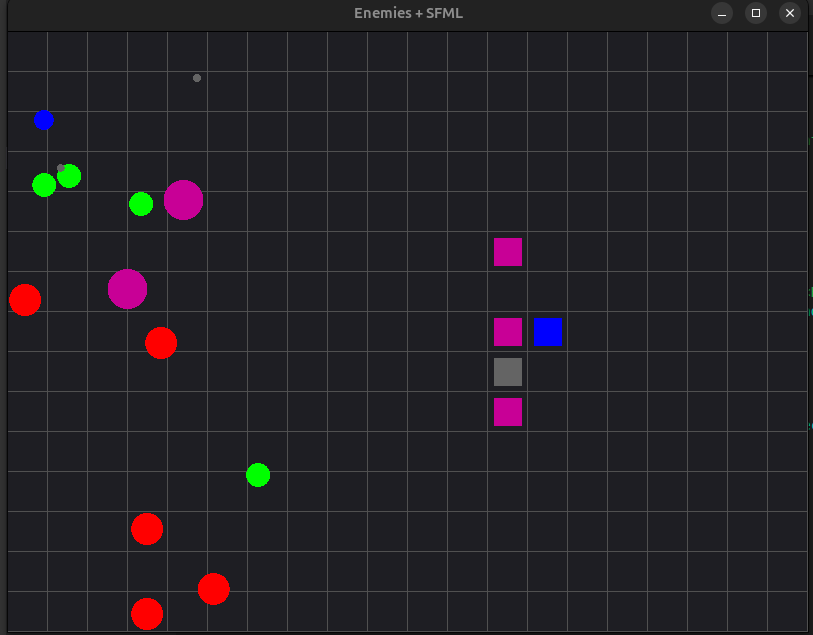
\includegraphics[width=0.7\textwidth]{figs/SFML1.png}}
    \caption{Rendu SFML avec les grilles, ennemis (ronds), tourelles (carrés)}
    \label{fig:exemple}
\end{figure}




\newpage

\subsection{Gestion du jeu}

Pour l’instant, j’ai créé les fonctions de génération d’ennemis et de tourelles.  
Les deux fonctions sont sensiblement identiques, à une différence près : dans ma fonction de génération de tourelles je prends en compte ce qui a été établi plus tôt avec les cellules.  

D’un clic de souris, je décide de poser une tourelle : le programme récupère les coordonnées de ma souris puis les compare avec celles d’une cellule.  
C’est cette fonction qui m’a posé le plus de problèmes : j’avais du mal à saisir quand on pouvait modifier une structure et quand on ne le pouvait pas.  
Je ne passais pas par référence pour mon tableau de cellules : lorsque je voulais poser une nouvelle tourelle sur une case déjà utilisée, le programme crashait ou n’appliquait pas mes changements.  
En passant par référence, j’ai pu corriger les problèmes et la fonction a fini par marcher.  

Je crée donc une sorte de « pointeur » nommé it qui agit sur la cellule correspondant à mon clic de souris. Référencer cells et it me permet de modifier les paramètres de la structure de cette cellule (par exemple la cellule avec l’id 27, donc la 27e cellule).  
Je peux ensuite établir deux conditions :  
- si ma cellule (id 27) possède déjà une tourelle (turreted == true), alors je ne fais rien ;  
- sinon, j’en génère une aléatoirement (pour le moment, c’est du test).  

\begin{figure}[h]
    \centering
    \makebox[\textwidth]{\includegraphics[width=1\textwidth]{figs/turreted1.png}}
    \caption{"game.cpp" – Classe Game, fonctions, generateTourelle}
    \label{fig:exemple}
\end{figure}

\newpage

\subsection{Progression personnelle}

Les différentes fonctions de mon programme (que vous pouvez retrouver sur GitHub dans la branche \texttt{test}) m’ont permis de mieux comprendre le fonctionnement du langage C++.  
Cette première ébauche d’un jeu de Tower Defense m’aura permis de poser les bases pour créer un jeu avec un code source propre, professionnel et exploitant les outils d’optimisation de C++. J'ai utilsé plusieurs outils pour m'aider dans mon apprentissage, notamment ChatGPT pour résoudre certaines erreurs de compilation et comprendre des concepts complexes (Je pense avant tout aux classes et leurs gestion).
Mais également la documentation officielle de SFML (\url{https://www.sfml-dev.org/documentation/2.5.1/}) pour comprendre les différentes fonctions et classes disponibles dans cette bibliothèque graphique. (exemple : la gestion des formes géométriques, des fenêtres, des événements, etc.) et enfin l'outils de développement Copilot de GitHub pour m'aider à écrire du code et gagner du temps.

\section{Conclusion des semaines 38-39}

Ces deux semaines ont été très formatrices pour nous deux. Nous avons pu approfondir nos connaissances en C++ et en SFML, tout en commençant à développer les bases de notre jeu Tower Defense. Nous avons également appris à travailler de manière autonome tout en collaborant efficacement. Notre prochain objectif est d'intégrer nos travaux respectifs pour créer un prototype jouable, en continuant à développer les fonctionnalités du jeu et en améliorant l'interaction entre les différentes classes. Si on se réfère au planning prévisionnel, nous sommes encore dans les temps pour finaliser le projet dans les délais impartis.